%
%\noindent
%\epigraph{The trees are in their autumn beauty,\\
%The woodland paths are dry,\\
%Under the October twilight the water\\
%Mirrors a still sky;\\
%Upon the brimming water among the stones\\
%Are nine-and-fifty swans.}{\textit{W.B. Yeats}}

Consider a curious TC: $X_{59}$, the ``Isogonal Conjugate of $X_{11}$'' \cite{etc}, i.e., the two centers have reciprocal trilinears.

Experimentally, $X_{59}$ is a continuous curve internally tangent to the EB at its four vertices, and with four self-intersections, Figure~\ref{fig:x59-center}, and as an animation \cite[PL\#12]{reznik2020-playlist-intriguing}. It intersects a line parallel to and infinitesimally away from either axis on six points, so its degree must be at least 6. Producing analytic expressions for salient aspects of its geometry has proven a tough nut to crack, namely, the following are unsolved:

\begin{itemize}
\item What is the degree of its implicit equation?
\item What is $t$ in $P_1(t)=\left(a\cos(t),b\sin(t)\right)$ such that $X_{59}$ is on one of the four self-intersections? For example, at $a/b=1.3$ (resp. $1.5$), $t$, given in degrees is ${\simeq}32.52^\circ$ (resp. $29.09^\circ$), Figure~\ref{fig:x59-center} (left-bottom).
\item What is $a/b$ such that if $X_{59}$ is on one of the lower self-intersection on the $y$-axis, the 3-periodic is a right triangle? Numerically, this occurs when $a/b=\alpha_{59}^\perp\,{\simeq}\,1.58$ and $t{\simeq}27.92^\circ$, Figure~\ref{fig:x59-center} (right).
\end{itemize}

\begin{figure}
    \centering
    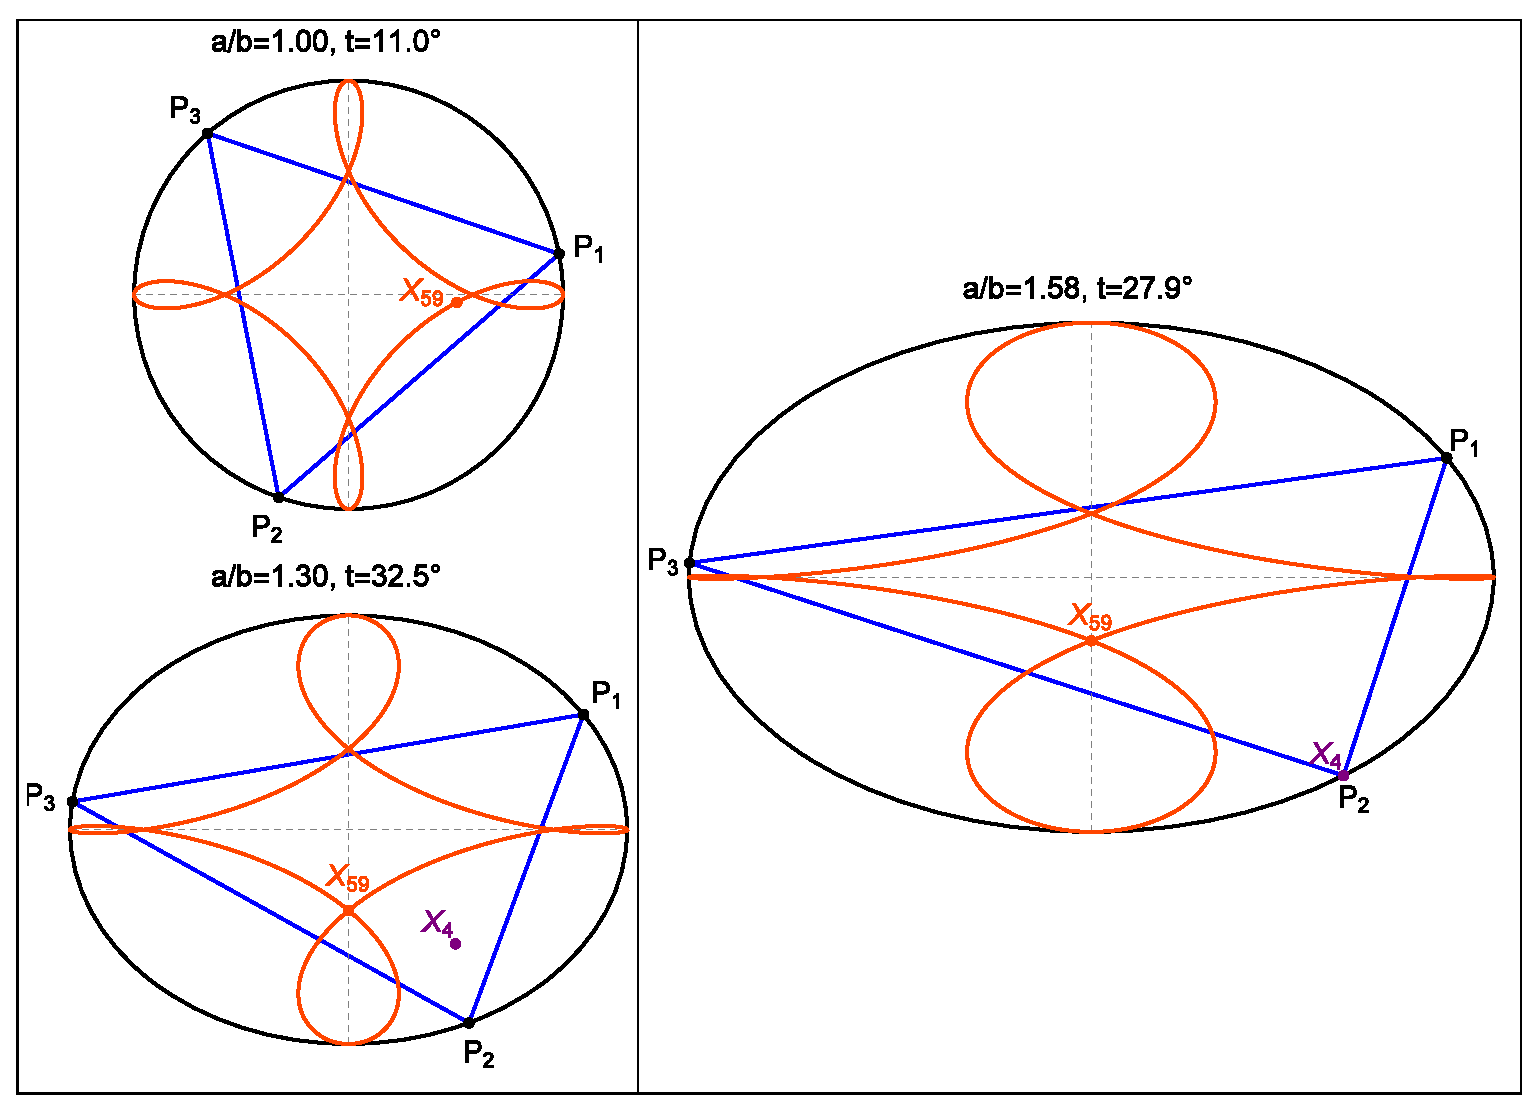
\includegraphics[width=.8\textwidth]{pics/1050_x59_center.eps}
    \caption{The locus of $X_{59}$ is a continuous curve with four self-intersections, and at least a sextic. It is tangent to the EB at its four vertices. \textbf{Top Left}: circular EB, $X_{59}$ is symmetric about either axis. \textbf{Bottom Left}: $a/b=1.3$, at $t{\simeq}32.5^\circ$ $X_{59}$ is at the lower self-intersection and the 3-periodic is acute ($X_4$ is interior). \textbf{Right}: at $a/b=\alpha_{59}^\perp\,{\simeq}\,1.58$ the following feat is possible: $X_{59}$ is at the lower self-intersection {\em and} the 3-periodic is a right-triangle ($X_4$ is on $P_2$). This occurs at $t{\simeq}27.9^\circ$. \textbf{Video}: \cite[PL\#12]{reznik2020-playlist-intriguing}}
    \label{fig:x59-center}
\end{figure}